
%----------------------------------------------------------------------------------------
%	PACKAGES AND OTHER DOCUMENT CONFIGURATIONS
%----------------------------------------------------------------------------------------

\documentclass[oneside, twocolumn]{article}

%\usepackage[sc]{mathpazo} % Use the Palatino font
%\usepackage[T1]{fontenc} % Use 8-bit encoding that has 256 glyphs
%\linespread{1.05} % Line spacing - Palatino needs more space between lines
%\usepackage{microtype} % Slightly tweak font spacing for aesthetics

\usepackage[english]{babel} % Language hyphenation and typographical rules
\usepackage{amsmath}
\usepackage[hmarginratio=1:1,top=32mm,columnsep=20pt]{geometry} \usepackage[hang, small,labelfont=bf,up,textfont=it,up]{caption}
\usepackage{booktabs}

\usepackage{xcolor}
\newcommand\myworries[1]{\textcolor{red}{#1}}
\newcommand\NumberOfGroups{43}
\newcommand\TotalHoursOfRecording{767}

\usepackage{enumitem}
\setlist[itemize]{noitemsep}

\usepackage{abstract}
\renewcommand{\abstractnamefont}{\normalfont\bfseries}
\renewcommand{\abstracttextfont}{\normalfont\small\itshape}

\usepackage{titlesec} % Allows customization of titles
%\renewcommand\thesection{\Roman{section}} % Roman numerals for the sections
%\renewcommand\thesubsection{\roman{subsection}} % roman numerals for subsections
%\titleformat{\section}[block]{\large\scshape\centering}{\thesection.}{1em}{} % Change the look of the section titles
%\titleformat{\subsection}[block]{\large}{\thesubsection.}{1em}{} % Change the look of the section titles

\usepackage{fancyhdr} % Headers and footers
\pagestyle{fancy} % All pages have headers and footers
\fancyhead{} % Blank out the default header
\fancyfoot{} % Blank out the default footer
\fancyfoot[RO,LE]{\thepage} % Custom footer text

\usepackage{titling} % Customizing the title section
\usepackage{hyperref} % For hyperlinks in the PDF
\hypersetup{colorlinks=false,linkbordercolor=red,linkcolor=green,pdfborderstyle={/S/U/W 1}}
\usepackage{graphicx}
\usepackage{epsfig}


%----------------------------------------------------------------------------------------
%	TITLE SECTION
%----------------------------------------------------------------------------------------

\setlength{\droptitle}{-4\baselineskip} % Move the title up

\pretitle{\begin{center}\Huge\bfseries} % Article title formatting
\posttitle{\end{center}} % Article title closing formatting
\title{\LARGE Thermset: A thermal-videos dataset of elder people bedrooms} % Article title
\author{Pablo Pusiol\\ \href{mailto:pdp0109@famaf.unc.edu.ar \qquad Pablo Pusiol }{pdp0109@famaf.unc.edu.ar} \and Federico Polacov \\\href{mailto:fdp0108@famaf.unc.edu.ar}{fdp0108@famaf.unc.edu.ar}}
\date{Universidad Nacional de C\'ordoba - FaMAF \\ \today}
%\date{\today} % Leave empty to omit a date
\renewcommand{\maketitlehookd}{%
%\begin{abstract}
%
%\end{abstract}
}

%----------------------------------------------------------------------------------------

\begin{document}
\maketitle

%----------------------------------------------------------------------------------------
%	ARTICLE CONTENTS
%----------------------------------------------------------------------------------------

\section{Introduction}
\label{sec:introduction}
Our interest is to automatically detect clinically relevant daily activities of seniors living independently or in nursing homes. To do that we will use thermal information and develop innovative computer vision technology. Modern computer vision is based on deep learning techniques and has proven to be very effective at automatizing visual recognition tasks such as detecting objects in images, tracking and detecting activities in videos, etc. A caveat of these techniques is the need of big amounts of labeled data for training their models. In practice, to achieve  models that could reliably work in new  environments (e.g. homes, people, etc.) would require of the training dataset to contain activity examples covering the full space of the manifold defined by all possible configurations of the target activities and environments.

While video cameras are traditionally used for daily activity monitoring, they need additional algorithms to overcome their inherent vulnerability to low light conditions, too much light, shadows, complex scenes. Far infrared sensors (thermal sensors) do not have any these issues because they create a crisp image based temperature data from a scene, so almost all the problems traditional RGB cameras face in processing and classifying images are avoided \cite{chengl}.

In this document, we introduce a new dataset: Thermset, an incremental dataset of thermal information recorded for different time intervals of (so far) 13\myworries{actualizar} senior citizens at their bedrooms with automatic annotations as described in \autoref{subsec:annotations}. Each of the instances of the dataset (videos) corresponds to a series of frames where each frame corresponds to the matrix of absolute temperature values captured by a far-infrarred sensor. The sensor captures for intervals of as little as 2 seconds or as long as 15 seconds. Until the date of writing this document, Thermset has about 767\myworries{actualizar} hours of recordings, where typical examples of data reflect an elder sleeping, wandering, getting ready to bed, receiving assistance from a caregiver. The dataset also contains thermal data of the different bedrooms with no people as shown in \autoref{fig:examples} Thermset is available through \url{http://forelderly.weebly.com/data}.

\begin{figure*}
  \centering
    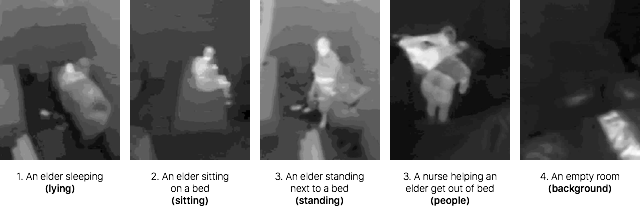
\includegraphics[width=1.0\textwidth]{images/examples}
  \caption{Examples of thermal data extracted from Thermset. (Images where stretched for easy reading)}
  \label{fig:examples}
\end{figure*}
%\textbf{Thermset in relation to other datasets}

%\textbf{Elderly activities datasets}

%\textbf{Thermal imaging datasets}

In \autoref{sec:technical} we provide technical details of how Thermset is structured, characteristics of data, annotations and how data is being gathered. The rest of the document is structured as follows: In \autoref{sec:properties} we provide qualitative information of the seniors recorded and environments and finally in \autoref{sec:application} we provide an example of how impactful Thermset can be to improve seniors wellbeing.

%------------------------------------------------

\section{Technical details}
\label{sec:technical}
\subsection{Structure}
Thermset is structured in groups. A group is a sequence of chunks with the same duration.
A chunk is represented with a sequence of thermal values matrixes expressed in Celsius degrees
(from now on we will call each thermal matrix a frame). Each group has chunks of a unique person
recorded for a certain time interval with a certain configuration of our recording tools as we will
describe in this section. Is important to notice that there is a time gap between each chunk of a
group. Its duration depends on the recording configuration used and is explained in \autoref{par:time-gap}.

Group names follow the structure \textbf{Name\_YYY}, where Name refers to an elder's alias and \textbf{YYY}
to the \textbf{YYY}-th group recorded of that elder. For instance, the group \textbf{Marge\_001} is the
1st group with recordings of an elder whose alias is Marge.

\subsection{Diversity of data}
Below we provide graphics to help understand better the distribution of the data collected. The majority of recordings were collected in nursing homes, but there are two groups recorded at two private addresses.

\myworries{grafico de porcentajes hombre/mujer}

\myworries{grafico de edades}

\myworries{grafico de largos de videos}

\subsection{Recording tools}
To record and create annotations we use Apple iOS devices and \href{http://www.flir.com/flirone/ios/}{FLIR One sensors}. The app used was \href{http://appstore.com/thermixforflirone}{Thermix}\cite{thermix} , available for free in the App Store.

We relied on 3 different devices to run Thermix: an iPod Touch 5th generation,
an iPhone 5 and an iPhone 5s. The far-infrared sensors used were Dongle and SLED versions of the FLIR One.
We configure Thermix in the iPhone 5 with an SLED sensor and in the iPhone 5s and the
iPod Touch with a dongle sensor\cite{sdk_flir_dongle}\cite{sdk_flir_sled}. Because Thermix excludes all frames during a sensor recalibration, we estimate the
average fps (frame per second) for each configuration achieving ~5fps, ~3fps and ~2fps respectively.
\myworries{CONTROLAR SI SE ENTIENDE}.

\subsubsection{Recording Configurations}
Groups in Thermset were recorded in different ways. Each of these are what we call \textit{Recording Configuration or RC}. There is a total of 7 Recording Configurations, labeled \textit{RC1} to \textit{RC8}. Information of the configuration and device/sensor used for each group is available at \url{http://forelderly.weebly.com/data}.  Below we describe 3 aspects of each configuration, and at \autoref{tab:1} we describe each Recording Configuration by this 3 aspects.

\paragraph{Precision of thermal data}
	For \textit{R = raw thermal data returned from the sensor} we construct a frame $F$, where $F(i,j)$ corresponds to the element $i,j$ of the frame adjusted by precision.

	\begin{itemize}
		\item \textbf{Low precision:}
			\[
			    F(i,j)=
			\begin{cases}
			    2 * R(i,j),		& \text{if } 1 \leq R(i,j) \leq 120\\
			    0,              & \text{O therwise}
			\end{cases}
			\]
			Where $R(i,j)$ is the temperature expressed in Celsius degrees with no decimal places. \textit{RC1, RC3} correspond to this precision.\\


		\item \textbf{High precision:}
			\[
			    F(i,j)=
			\begin{cases}
			    round(2 * R(i,j)),		& \text{if } 1 \leq R(i,j) \leq 120\\
			    0,              & \text{Otherwise}
			\end{cases}
			\]
			Where $R(i,j)$ is the temperature expressed in Celsius degrees with one decimal place. The $round$ function returns the integral value nearest to its argument, rounding half-way cases away from zero.
	\end{itemize}

\paragraph{Video lenght}
Each group records videos for a certain number of time that ranges between 2 and 15 seconds. The amount of frames per video is related to the fps the device is capable of and the time each device was recording for:
	\begin{equation}
	\resizebox{.423 \textwidth}{!}{$number\_of\_frames = fps(device) * video\_lenght(RC)$}
	\end{equation}


\paragraph{Dead intervals}
\label{par:time-gap}
Thermix records and uploads small chunks of video to the cloud. There are two possible configurations: either Thermix saves chunks to the device disk continuously (continuous mode) or waits until a chunk is sent to start recording the next one (one-by-one mode).
\begin{itemize}
	\item \textbf{Continuous mode:}\\
		Video chunks in groups recorded with continuous mode are separated by a small time window (between 2 and 5 seconds in average), that correspond to the time Thermix takes to compose the chunk\footnote{The composition of the chunk consists in generating a video from thermal data and annotating the first thermal frame using the method described in \autoref{sec:application}}. This means, Thermix did not wait for a video chunk to be sent before start recording the next one.\\
	\item \textbf{One-by-one mode:}\\
		Videos in groups recorded with one-by-one mode are separated by the time Thermix takes to compose the video chunk as in continuos mode plus the time the device takes to upload it to the cloud.
\end{itemize} \myworries{$\leftarrow$ revisar no me gusta}

\begin{table*}[t]
  \centering
\begin{tabular}{c*{4}{c}}
\hline
\textbf{RC} & Video lenght & Precision of thermal data & Sampling dead intervals\\
\hline
\textbf{1} & 10 seconds & Low precision 		& One-by-one \\
\textbf{2} & 15 seconds & Low precision 		& Continuous \\
\textbf{3} & 15 seconds & Low precision 		& Continuous \\
\textbf{4} & 10 seconds & High precision 	& One-by-one \\
\textbf{5} & 2 seconds  & High precision 	& One-by-one \\
\textbf{6} & 2 seconds  & High precision 	& One-by-one \\
\textbf{7} & 5 seconds  & High precision 	& One-by-one \\
\textbf{8} & 5 seconds  & High precision 	& One-by-one \\
\hline
\end{tabular}
  \caption{Details of recording configurations comprehended by Themset}
  \label{tab:1}
\end{table*}

\subsection{Annotations}
\label{subsec:annotations}
Thermset provides automatic annotations generated by Thermix for each video. The annotation corresponds to the output of the classification of the first frame of the video using the method described at \autoref{sec:application}. Classes are background, standing, sitting, lying and people. Annotations for each group are listed on file (named \textbf{GROUP\_NAME}\_annotations.txt) stored in each group folder. Annotations follow the structure:

	\textit{video\_url \textbraceleft \textless class\_id:score \textgreater}\textbraceright \textsuperscript{5},

	where \textit{class\_id} corresponds to classes as detailed in \autoref{tab:2}, and \textit{score} correspond to the output of the classification each \textit{class\_id}.
  An example of an annotation is shown in \autoref{fig:image_w_annotation}.
\begin{table}
\center
	\begin{tabular}{l | l}
\textit{id} & \textit{class} \\
\hline
1 & lying \\
2 & sitting \\
3 & standing \\
4 & group \\
5 & background \\
\end{tabular}
  \caption{Classes and their corresponding ids.}
  \label{tab:2}
\end{table}

\begin{figure}
  \centering
    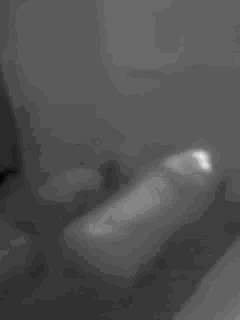
\includegraphics[width=0.25\textwidth]{images/image_with_annotation.png}
  \caption{Frame with annotation: \\2016-09-06\_03.53.33 1:0.998713 4:0.000638 2:0.000534 5:0.000074 3:0.000040}
  \label{fig:image_w_annotation}
\end{figure}

\begin{figure*}
  \centering
    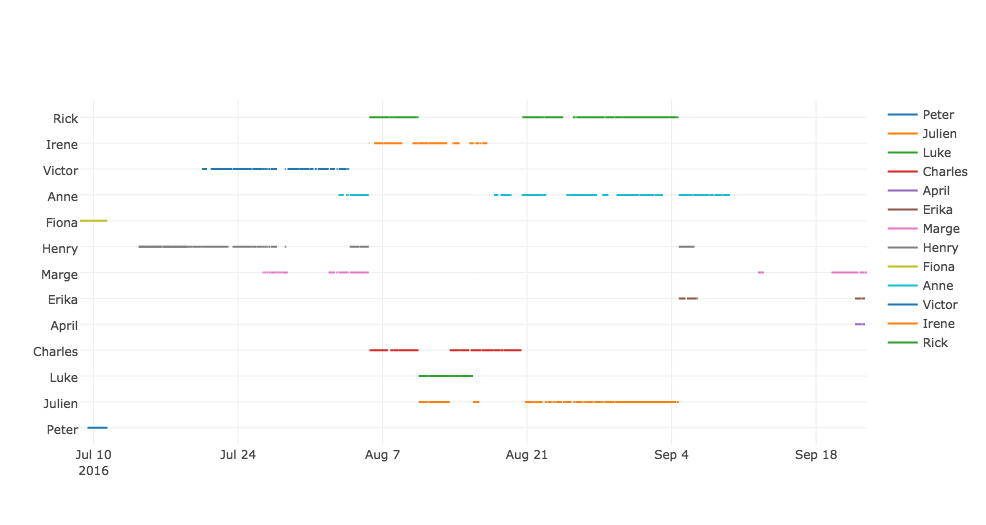
\includegraphics[width=1.0\textwidth]{images/recording_timeline}
  \caption{Distribution in time of recordings per elder. Blank spaces represent a group change or intervals where the system was not recording for more than 5 minutes}
  \label{fig:timeline}
\end{figure*}

%------------------------------------------------

\section{Qualitative description of the dataset}
\label{sec:properties}
\paragraph{Recording environments}
Videos where recorded at several bedrooms in 2 different nursing home facilities and at 2 private homes. All videos where recorded during winter.
\paragraph{About the people}
Until the date of writing this document, Thermset has data of the following elders:
\begin{itemize}
	\item \textbf{Marge:} 90+ years old, Female \\
			\underline{Diseases or disabilities:} Hyperthyroidism. Had fractures due to falls \\
			\underline{Situation:} Living at a healthcare facility. Shares the bedroom with another person. Takes naps daily. Sleeps with a diaper. Had a hip fracture after a fall. Moves around with walker and she’s afraid of walking alone. Requires constant assistance for moving, entering, leaving bed, etc. \\
	\item \textbf{Peter:} 80+ years old, Male \\
			\underline{Diseases or disabilities:} Had fractures due to falls \\
			\underline{Situation:} Lives at his place, alone. He does not require assistance, but due to a knee fracture has difficulties to move. Uses a walking stick. Takes naps and reads the newspaper while in bed. \\
	\item \textbf{Anne:} 60+ years old, Female \\
			\underline{Diseases or disabilities:} Alzheimer’s \\
			\underline{Situation:} Living at a healthcare facility. Shares the bedroom with another person. Wanders during the day. \\
	\item \textbf{Henry:} 55+ years old,  Male \\
		  	\underline{Diseases or disabilities:} Vascular dementia \\
		  	\underline{Situation:} Living at a healthcare facility. Shares the bedroom with Victor. Wanders frequently during the day. \\

	\item \textbf{Victor:} 80+ years old, Male \\
			\underline{Diseases or disabilities:} Visual impairment \\
			\underline{Situation:} Living at a healthcare facility. Shares the bedroom with Henry. Takes frequent naps during daytime. Due to his visual impairment requires frequent assistance but he uses a snub to urinate next to his bed without assistance. Urinates frequently. \\
	\item \textbf{Fiona:} 75+ years old, Female \\
			\underline{Diseases or  disabilities:} Overweight, Hyperthyroidism \\
			\underline{Situation:} Lives at her place, alone. She does not require assistance. Takes naps and watches TV while in bed. \\
	\item \textbf{Irene:} 75+ years old, Female \\
			\underline{Diseases or  disabilities:} Advanced Alzheimer's disease \\
			\underline{Situation:} Living at a healthcare facility. Shares the bedroom with  Anne. Due to her incapacity of moving by herself, requires a wheelchair. Sleeps in  a special bed to prevent falls. \\
	\item \textbf{Charles:} 70+ years old, Male \\
			\underline{Diseases or  disabilities:}  Schizophrenia, Alcoholism \\
			\underline{Situation:} Living at a healthcare facility. Shares the bedroom with two other male elders. Wanders during the day but has no major mobility issues. \\
	\item \textbf{Rick:} 75+ years old, Male \\
			\underline{Diseases or  disabilities:} Visual impairment, Vascular dementia,  Limited mobility. \\
			\underline{Situation:} Living at a healthcare facility. Shares bedroom with Henry and Victor. Requires assistance to move but uses a snub to urinate next to his bed without assistance \\
	\item \textbf{Julien:} 90+ years old, Male \\
			\underline{Diseases or disabilities:} Alzheimer's   disease, mild arthritis \\
			\underline{Situation:} Living at a healthcare facility. Shares the bedroom with Charles and Luke. Does not require assistance to move.  Does hydrotherapy to  combat arthritis. \\
	\item \textbf{Luke:} 80+ years old, Male \\
			\underline{Diseases or disabilities:} Alzheimer's disease \\
			\underline{Situation:} Living at a healthcare facility. Shares the bedroom with Charles and Julien. Does not require assistance to move.\\
	\item \textbf{Erika:} 70+ years old, Female \\
			\underline{Diseases or disabilities:} Senile dementia \\
			\underline{Situation:} Living at a healthcare facility. Shares the bedroom with 2 other women. Requires full-time assistance.\\
	\item \textbf{April:} 70+ years old, Female \\
			\underline{Diseases or disabilities:} Senile dementia \\
			\underline{Situation:} Living at a healthcare facility. Shares the bedroom with 2 other women. Due muscular spasms product of her advanced dementia requires full-time assistance. \\
\end{itemize}

%------------------------------------------------

\section{Application: Pose estimation}
\label{sec:application}

In the context of daily activities detection, collecting a training set large enough to accurately detect clinically relevant activities is hard. It might require of hundreds of data feeds for several days, or years if we consider the environmental temperature fluctuations and the different appearances (e.g. clothes) that a person will have during the stations. In addition, it would require of several human annotators working 24/7 watching and extracting the target activities appearing in the streams. Likely, the number of labelers would be proportional to the number of data streams that need to be analyzed. In addition to the complexity of collecting a big labeled  training  dataset, the size of each labeled example could present a problem as well. Optimizing an utility function over long-term visual streams would require a massive amount of computing power and memory.

To overcome the limitations described above, instead of thinking in rigid models to detect all activities at once it is more convenient to design dynamic systems capable of learning incrementally new activities when new labeled data arrives.  Daily living activities are hierarchically composed of sub-activities occurring in a variable period of time. In general, the deeper we move in the taxonomy of activities, the less training-data is needed for building reliable models to detect them. This observation is related to the lower dimensionality of their manifold in comparison with more complex activities. We are interested in detecting complex activities in incremental bottom-up steps. First, by detecting anchoring activities lying at the lower end of the human activities taxonomy. These anchor activities are persistent human features appearing as sub-activities of more complex ones.  Enabling a robust detection of these anchors will enable our second stage of learning, which will use the anchors for detecting and analyzing complex long-term human activity.  For the rest of this section we will focus in the first stage of our algorithm: defining and modeling the detection of anchoring activities.\\

\textbf{Pose Anchors} One of our anchor activities is the detection of pose. Human pose  is a highly descriptive and persistent feature, capable  of  characterizing complex activities. For senior adults living independently, changes of pose in the particular contexts could be describing a high risk situation. For  example,  a person changes from "standing" to "lying in the floor" could indicate the  occurrence  of a fall. In nursing-homes, detecting and alerting the "coming out of bed" could enable promptly caregiver's assistance.

The detection of pose anchors is connected to the monitoring of clinically relevant activities. Here we borrow some of the target daily living  activities  described in \cite{pac_stanford}, where several of the activities presented there can be inferred directly from the human pose.
​
For example:
\begin{enumerate}
	\item \textbf{Falls:} corresponds to transitions from standing to lying or from sitting to lying -as long as lying is not happening in the bed area
	\item \textbf{Front-door-Loitering:} corresponds to detecting a person standing in selected locations
	\item \textbf{Day-Night-Reversals and night wanders:} corresponds to detecting a person standing at unusual night hours
	\item \textbf{Sleep:} corresponds to detecting a person lying in bed, even when the person is covered by a blanket
	\item \textbf{Immobility (bed or chair):} corresponds to long periods of time where the person is either sitting or lying (in bed)
	\item \textbf{Restlessness:} corresponds to detecting and tracking pose changes for long periods of time where the person is perpetually agitated or in motion.
\end{enumerate}

\subsection{Model}

We built our model as a Fully Convolutional Network derived Matt Zeiler's model \cite{zeiler-2014}, which takes an input of 225x255x3 thermal image is convolved through 5 layers. The last layer is fully connected, taking features from the top convolutional layer as input in vector. The final layer is a 5-way softmax function, 5 being the number of classes: \textit{lying}, \textit{sitting}, \textit{standing}, \textit{group} and \textit{background}. All filters and feature maps are square in shape.

\subsection{Dataset}
The dataset used to train this model was labelled manually and contains 30825 frames with 6165 frames by class, where 12726 were selected from Thermset videos and 18099 where collected from a controlled environment.

We randomly split 80\%/20\% of data into training and testing datasets. Since our training units are videos, we are careful of not including any frame of a testing video in the training set (and vice versa)

\subsection{Evaluation}
The dataset was split into training and validation datasets,  80\%/20\% respectively. We are careful of not including any frame of a testing video in the validation set (and vice versa). Training was done for 500 epochs with a Dropout rate of 0.5. Results were obtained running the algorithm in the validaation dataset with a generalization error of  7.09\%. Our loss function is cross entropy for logits. (See \autoref{fig:cross_entropy_42}).

\begin{figure}
  \centering
    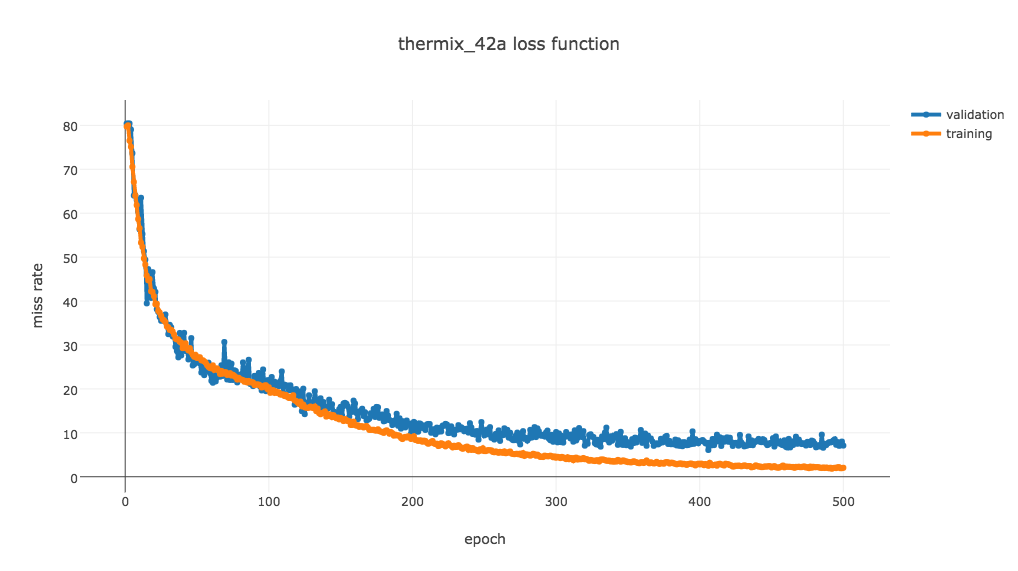
\includegraphics[width=0.5\textwidth]{images/loss_42.png}
  \caption{Cross entropy loss for logits}
  \label{fig:cross_entropy_42}
\end{figure}

\iffalse
\begin{figure}
  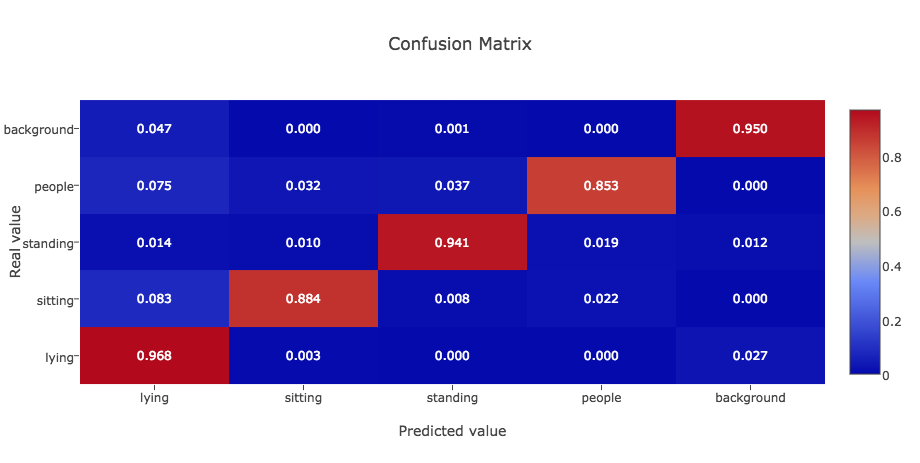
\includegraphics[width=0.5\textwidth]{images/confusion_matrix_42.png}
  \caption{Confusion matrix}
  \label{fig:confusion_matrix_42}
\end{figure}
\fi

\iffalse
\paragraph{Using the model for presence detection}
On the 20\% of data left out of training, shown above as validation data, our model  achieves the following evaluation metrics, where positive is presence of at least a person in the scene:

\begin{itemize}
	\item ​\textbf{accuracy:} 98.20 \%
	\item ​\textbf{sensitivity:} 98.97 \%
	\item ​\textbf{specificity:} 95.05 \%
	\item ​\textbf{precision:} 98.78 \%
	\item ​\textbf{negative predictive value:} 95.81 \%
	\item ​\textbf{fall-out:} 4.95 \%
	\item ​\textbf{miss-rate:} 1.03 \%
	\item ​\textbf{false-discovery-rate:} 1.22 \%
\end{itemize}
\fi

Thermix provides a publicly available account where this model is being used live for presence detection for 3 people living in a nursing home, this helps nursing home staff to monitor activity in those scenes. Access can be requested via \url{http://forelderly.weebly.com/data}.

%------------------------------------------------

\section{Discussion and further work}

\subsection{Extending Thermset}
\paragraph{Annotations}
Thermset provides automatic annotations created using the procedure explained at \autoref{sec:application}. To train the model, we labelled 30825 frames. Creating different ground truths, such as localization of people would allow a better understanding of the scene.
\paragraph{Size}
Thermix provides a plug-and-play interface to easily gather thermal data. So far we collected 767\myworries{actualizar} hours of recordings of 13\myworries{actualizar} seniors. At the moment of writing this document, Thermix is set up in three different locations and we have plans of augmenting the dataset with more seniors in different locations.

\paragraph{Exploiting Thermset}
Thermset provides hours of recordings of seniors being aided, sitting, wandering, people that felt to the ground, nurses, etc. Such data is highly valuable for training new algorithms aimed to help the elderly live better and benchmarking existing algorithms in real life situations.
%------------------------------------------------
\paragraph{Acknowledgement}
The authors would like to like to thank all the nurses and doctors at the healthcare facilities from where we collected the data. Thank also Professor Jorge Sanchez from National University of C\'ordoba for his helpful remarks.

%----------------------------------------------------------------------------------------
%	REFERENCE LIST
%----------------------------------------------------------------------------------------

\begin{thebibliography}{99}

\bibitem{chengl} Hong Chengl, Zicheng Liu, Yang Zhaol, Guo Yel  {\em Real world activity summary for senior home monitoring.}  2011.
\bibitem{sdk_flir}FLIR One SDK, {\url{http://developer.flir.com/sdk-documentation/}}, accessed August 2016.
\bibitem{sdk_flir_sled}FLIR One SLED Tech Specs, {\url{http://www.flir.com/flirone/press/FLIRONE_Fast_Facts_Tech_Specs.pdf}}, accessed August 2016.
\bibitem{sdk_flir_dongle}FLIR One Dongle Tech Specs, {\url{http://www.flirmedia.com/flir-instruments/industrial/datasheets/flir-one-datasheet.html}}, accessed August 2016.
\bibitem{thermix}Thermix for FLIR One, {\url{https://appstore.com/thermixforflirone/}}, accessed August 2016.
\bibitem{pac_stanford} Stanford PAC Seniorcare website, {\url{http://vision.stanford.edu/pac/seniorcare/}}, accessed August 2016.
\bibitem{zeiler-2014} Matthew D. Zeiler and Rob Fergus {\em Visualizing and Understanding Convolutional Networks}, ECCV 2014

\end{thebibliography}

%----------------------------------------------------------------------------------------

\end{document}
